% tex for data

\documentclass{scrartcl}
\usepackage{url,graphicx,tabularx,array,amsmath,amssymb,amsthm,booktabs,float}
\usepackage[margin=.65in, top=.5in, bottom=.8in]{geometry}
\usepackage[toc,page]{appendix}
\graphicspath{{C:/Users/Colin/Documents/GitHub/533-proj/}{C:\Users}}
\title{Failure Time Distribution Estimation with Backblaze Hard Drive Data}
\subtitle{Stat 533 Class Project}
\author{Colin Lewis-Beck\\
  \and
  Eric Mittman}
\begin{document}
\noindent
\maketitle
\section*{Data}
The data analyzed is hard drive testing data from the company, Backblaze\cite{backblaze}.  Since 2013, Backblaze has been continuously spinning hard drives in controlled storage pods.  Hard drives are run until they fail or are right censored.  When a hard drive fails it is permanently removed from testing.  In addition, new hard drives are regularly added to the testing sample.  We downloaded the latest data published by Backblaze dating from January 1, 2015 to September 30, 2015.  Blackblaze provides over 70 variables on each hard drive; we will focus on only the following subset: an indicator variable for the last day the hard drive was in service before failing, the number of hours a hard drive has been on test, and the model/brand of each hard drive.

The raw data we downloaded from Backblaze contained 54,398 unique drives.  Because we are interested in making comparisons among models, we excluded models with fewer than 100 drives in testing.  Also, drives that failed in fewer than 20 days were removed; we justify excluding these data for the reason that they represent a failure mode that is not of interest.

There were some other bizarre observations in the data; for example, hard drives listed as being in test for over 10 years or drives that entered and exited the sample on the same day.  These bizarre observations were likely due to mis-coding and were dropped.  After cleaning the data we had a sample size of 52,811 total drives for analysis.

The final sample included 21 hard drive models.  Below is a summary of the distribution of failures, and total testing time for each model.  The total number of failures was 1030.  The majority of those failures came from models 5, 7, 9, and 11.  Not surprising, model 11, which had the most failures also had the longest total testing time; however, this relationship was not uniform across models.  Model 1 had the 2nd longest total testing time, but relatively few failures.

\begin{figure}[H]
\centering
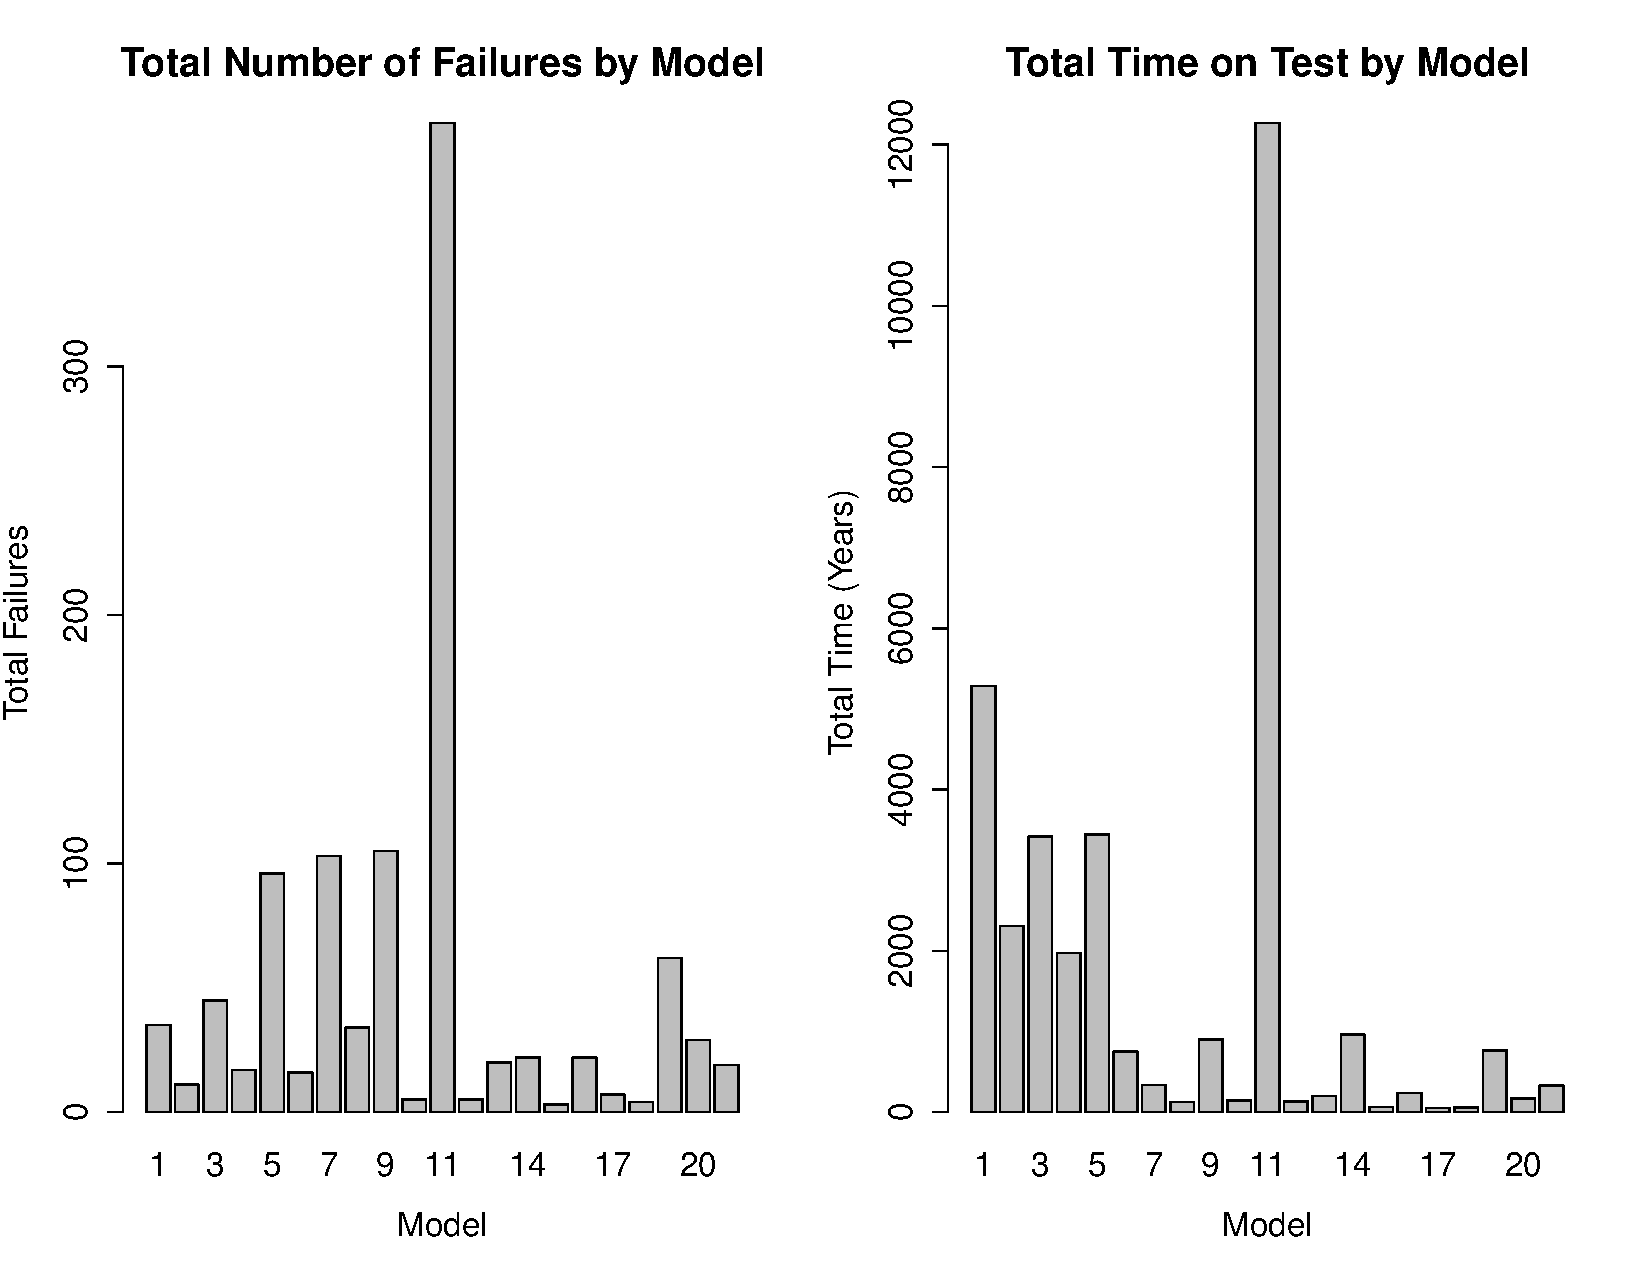
\includegraphics[height=7.5cm]{sumstat1.pdf}
\end{figure}
We also examined the distribution of failure times.  The shape is slightly skewed to the right with the majority of failures occurring within 250 days. However, with over 50,000 of the hard drives start times left truncated it is specious to infer that the failure times suffer from infant mortality.   
\begin{figure}[H]
\centering
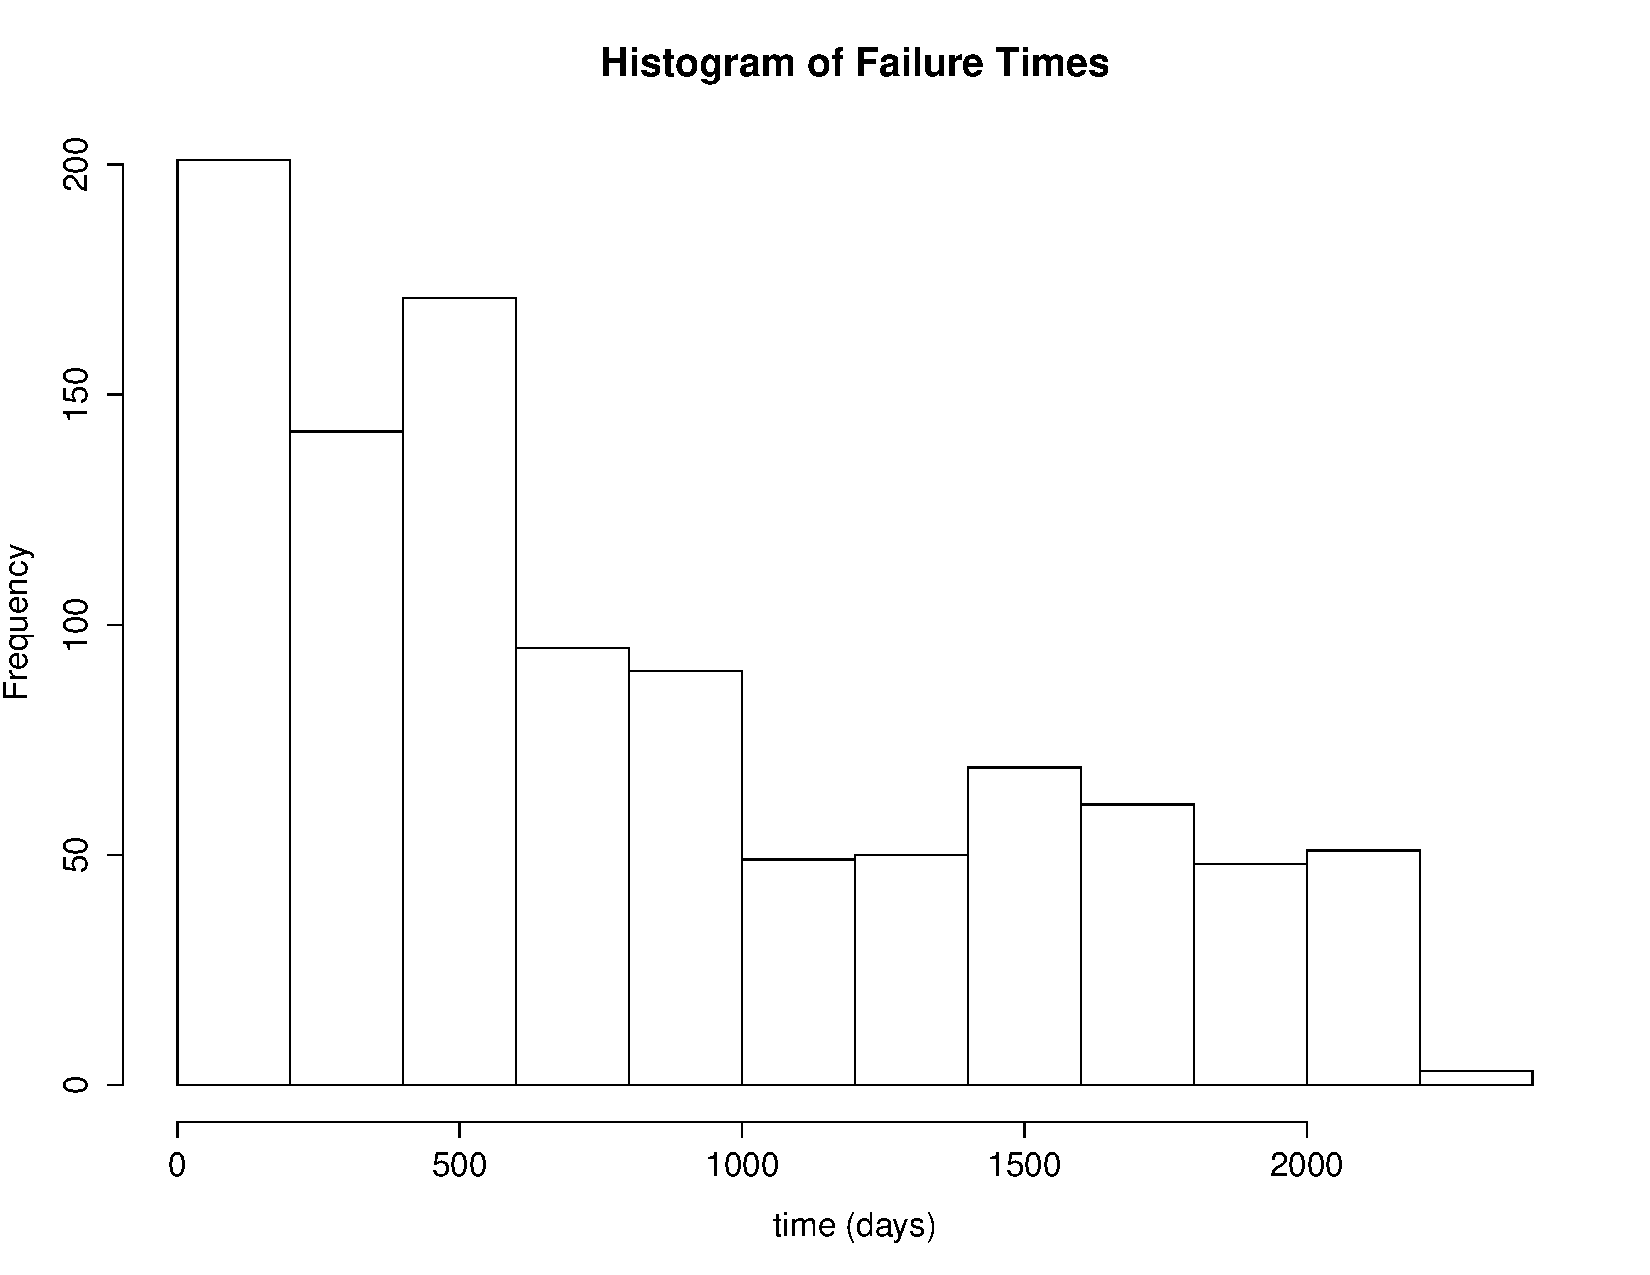
\includegraphics[height=8cm]{failhist.pdf}
\end{figure}

\section*{Model}
We used a Bayesian modeling approach to estimate the Weibull parameters for each model. Rather than modeling each model independently, we modeled the Weibull parameters hierarchically, to pool information and to provide better inferences, particularly for the brands that produced few failures. The model was fit using the rstan package in R \cite{stan}.\\

We parameterized the Weibull in terms of a lower log quantile, $t_p$ (where $p=0.01$), and scale, $\sigma$. These were modeled by a Student's t with 5 degrees of freedom and a lognormal, respectively.

\[Y_{mi} \stackrel{ind.}{\sim} \operatorname{Weibull}(\eta_m, \beta_m)\]
\[\sigma_m = \frac{1}{\beta_m}, \quad t_{p,m} = \exp\{\log(\eta_m) + \sigma_m \Phi_{sev}(p)\}\]
\[\log(t_{p,m}) \stackrel{i.i.d}{\sim} \operatorname{t}(\nu = 5, \mu_1, \tau_1)\]
\[\sigma_m \stackrel{i.i.d}{\sim} \operatorname{log-normal}(\mu_2, \tau^2_2)\]

The following uninformative and vague priors were used for the hyperparameters.
\[p(\mu_1,\mu_2) \propto 1\]
\[\tau_1,\tau_2 \stackrel{ind.}{\sim} \operatorname{half-Cauchy}(0,10)\]

The model for $Y_{mi}$ must be modified to accommodate the censoring and truncation patterns in the data. In the case of a failure that was observed and left-censored at $t_L$,
\[Y_{mi} \sim \operatorname{TWeibull}(\eta_m, \beta_m, t_L, \infty),\]
where $\operatorname{TWeibull}(\eta,\beta,a,b)$ is a truncated Weibull distribution with left and right truncation points a and b, respectively. For untruncated, right censored observations with censoring point $t_c$,
\[Y_{mi} \sim \operatorname{Bernoulli}(1-\Phi(t_c)),\]
where $\Phi$ is the cdf for a $\operatorname{Weibull}(\eta_m,\beta_m)$ distribution.
For observations that are both right censored and truncated,
\[Y_{mi} \sim \operatorname{Bernoulii}(1-\Phi_{t_L}(t_c)),\]
where $\Phi_{t_L}$ is the cdf for a left truncated Weibull distribution. 

\section*{Results}
Stan's Hamiltonian MCMC simulates posterior distributions for each model's parameters.  Since $\eta$ is extremely far away from the majority of the data we focus on the posterior distribution of $t_p$ (where $p=0.01$) and $\beta$.  The plot below shows the median of the posterior estimate (in hours) along with error bars corresponding to the middle 50\% of the distribution.  Just focusing on the medians, there are differences in reliability across the hard drive brands: Model 2 takes the longest time to reach the .01 quantile, whereas Model 13 is the fastest.  Yet after taking into account the uncertainty around the medians, most differences are no longer statistically significant as the majority of the credible intervals overlap. Owing to greater posterior precision, we can reasonably claim that it is probable that models 11 and 14 reach 1\% failing slower than models 7, 8, 9, 12, 13, 15, 16, 17, 19 and 21.
\begin{figure}[H]
\centering
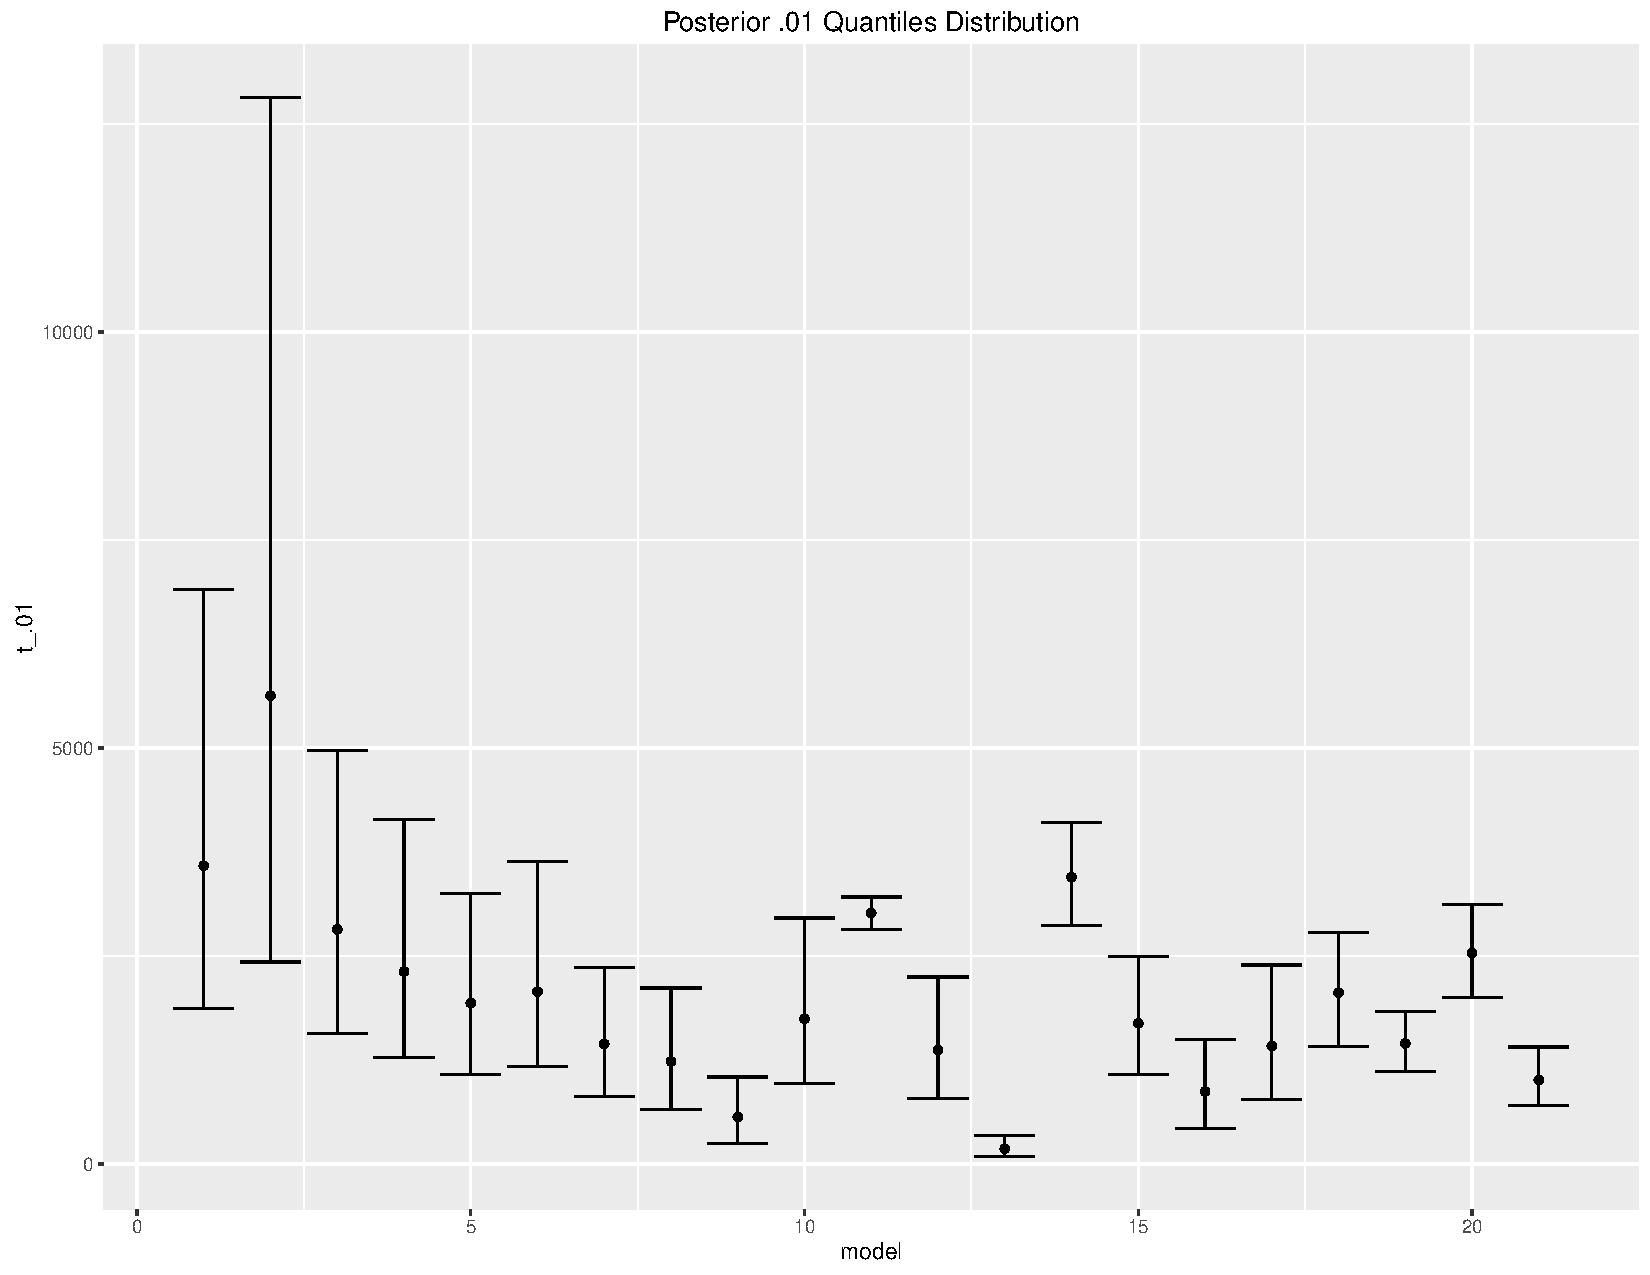
\includegraphics[height=8cm]{postquant.pdf}
\end{figure}

We can also compare the posteriors of estimated $\beta$ across models.  A line at $\beta=1$ seperates models with infant mortality versus those with an increasing hazard function.  Again, with so few failures, these results have large credible intervals; however, it does appear that Model 20 has a $\beta$ greater than 1 while Models 1 and 13 have hard drives that suffer from early failures.
\begin{figure}[H]
\centering
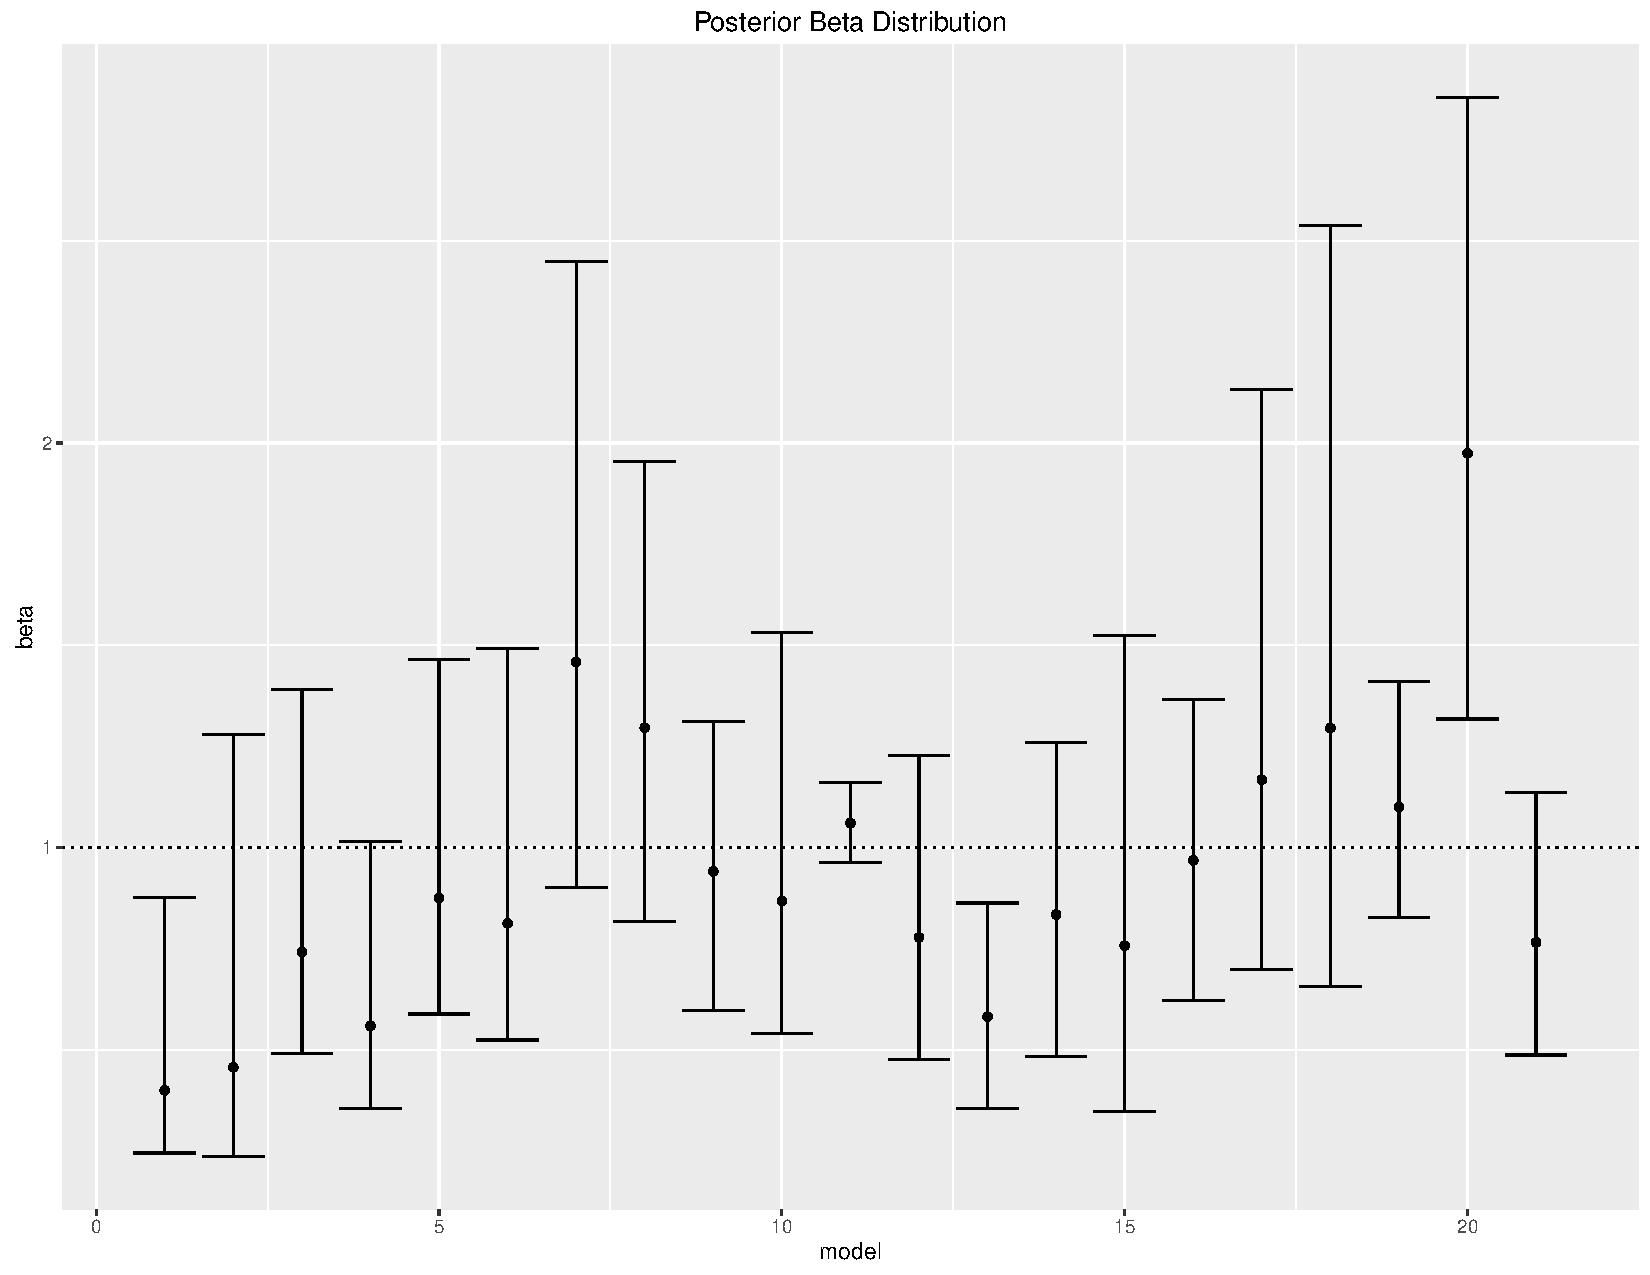
\includegraphics[height=8cm]{postbeta.pdf}
\end{figure}

Finally, to assess model fit, we overlay the fitted models with an 80\% credible interval ribbon on top of the left truncated adjusted Kaplan-Meier non-parametric estimate \cite{meeker2014statistical}.  The empirical CDF is on the y-axis; the x-axis is in terms of hours.  Looking at Model 1 and Model 11 we can see the Weibull model captures the data quite well.  It appears the credible interval for Model 1 is quite wide; however, the ribbon only covers a narrow range of about .01--and it should be noted that Model 1 only had 22 failures.  In contrast, Model 11 had 381 failures, and as expected the credible interval is thin with the data points hovering in the middle.

\begin{figure}[H]
  \centering
  \begin{minipage}[b]{0.4\textwidth}
    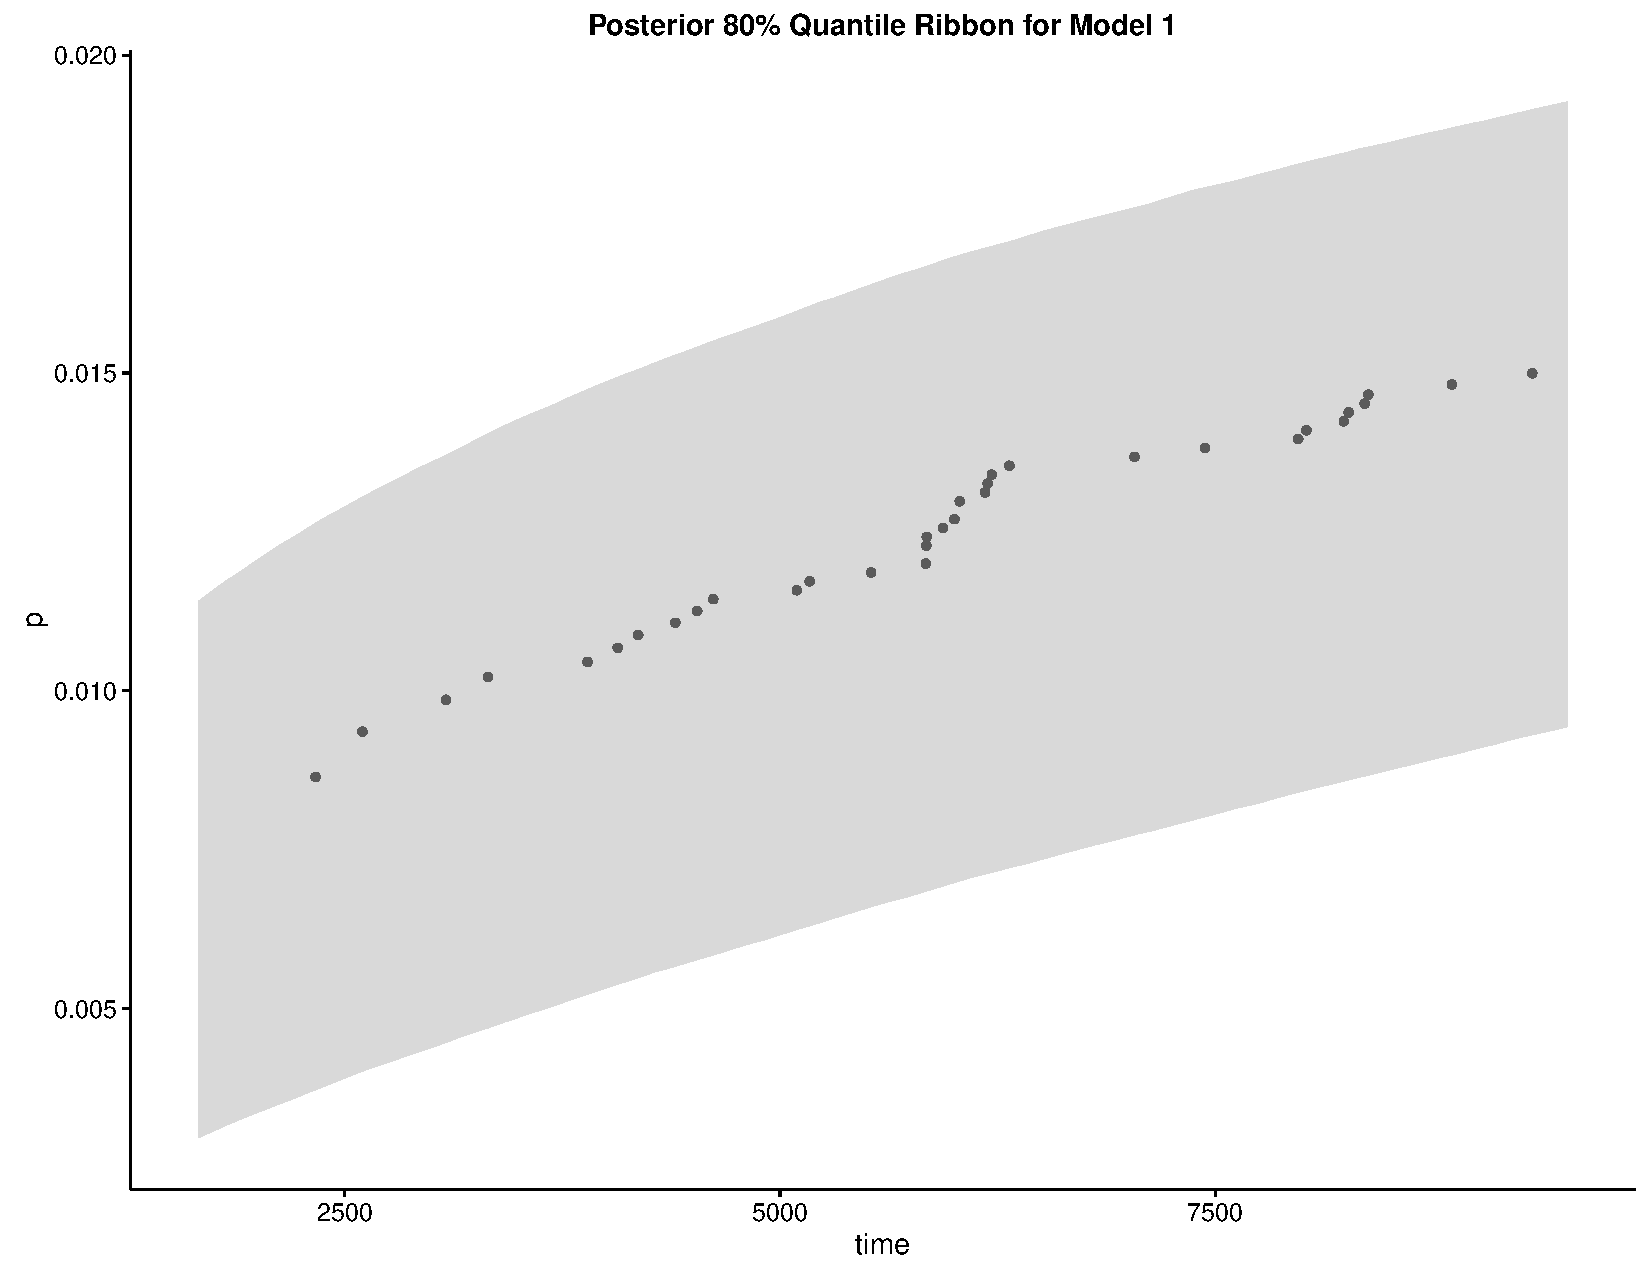
\includegraphics[width=\textwidth]{plot1.pdf}
  \end{minipage}
  \hfill
  \begin{minipage}[b]{0.4\textwidth}
    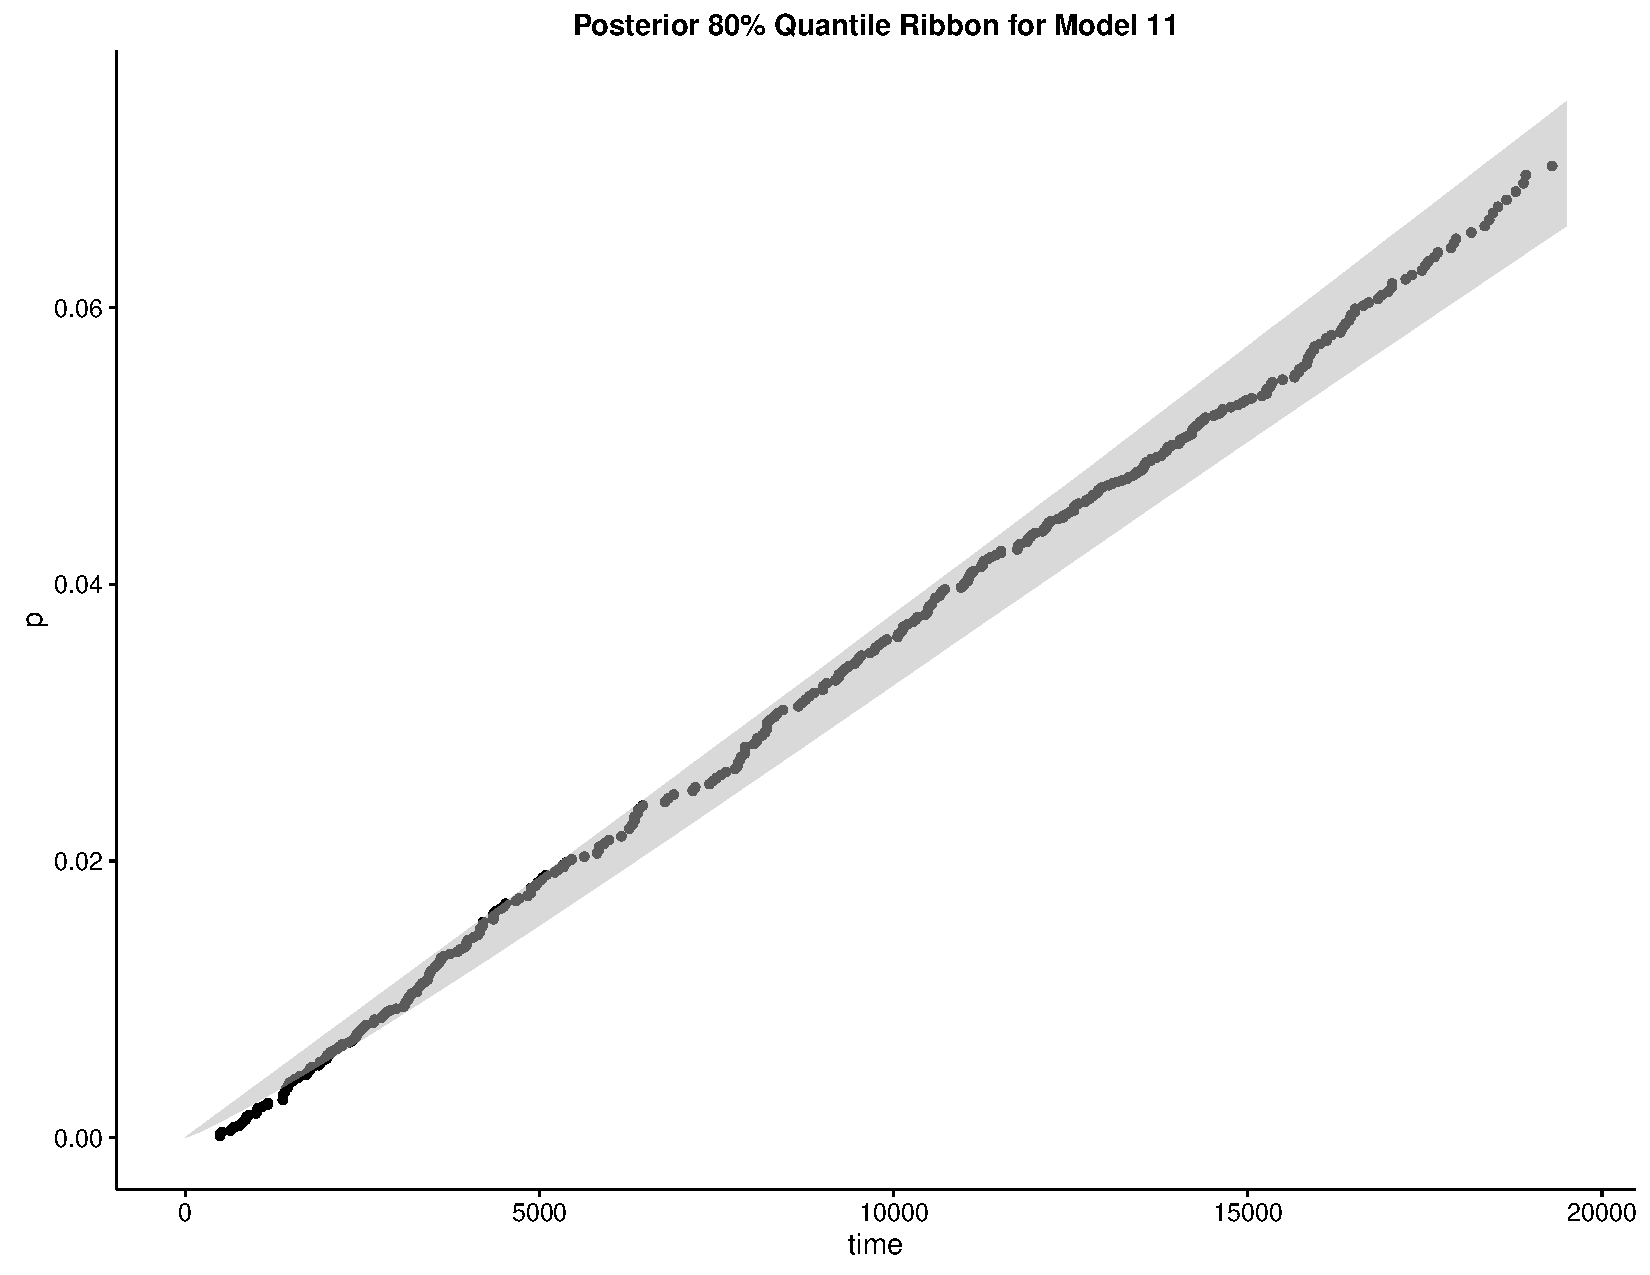
\includegraphics[width=\textwidth]{plot2.pdf}
  \end{minipage}
\end{figure}

Some hard drive brands were not modeled as well.  Model 15 only had 3 failures and seen below the credible interval does not capture all of the data.  Model 21 had a cluster of failures at around 1000 hours that were not picked up in the model.  Again, though, with only 19 failures there is very little data to accurately model the failure distribution.  

\begin{figure}[H]
  \centering
  \begin{minipage}[b]{0.4\textwidth}
    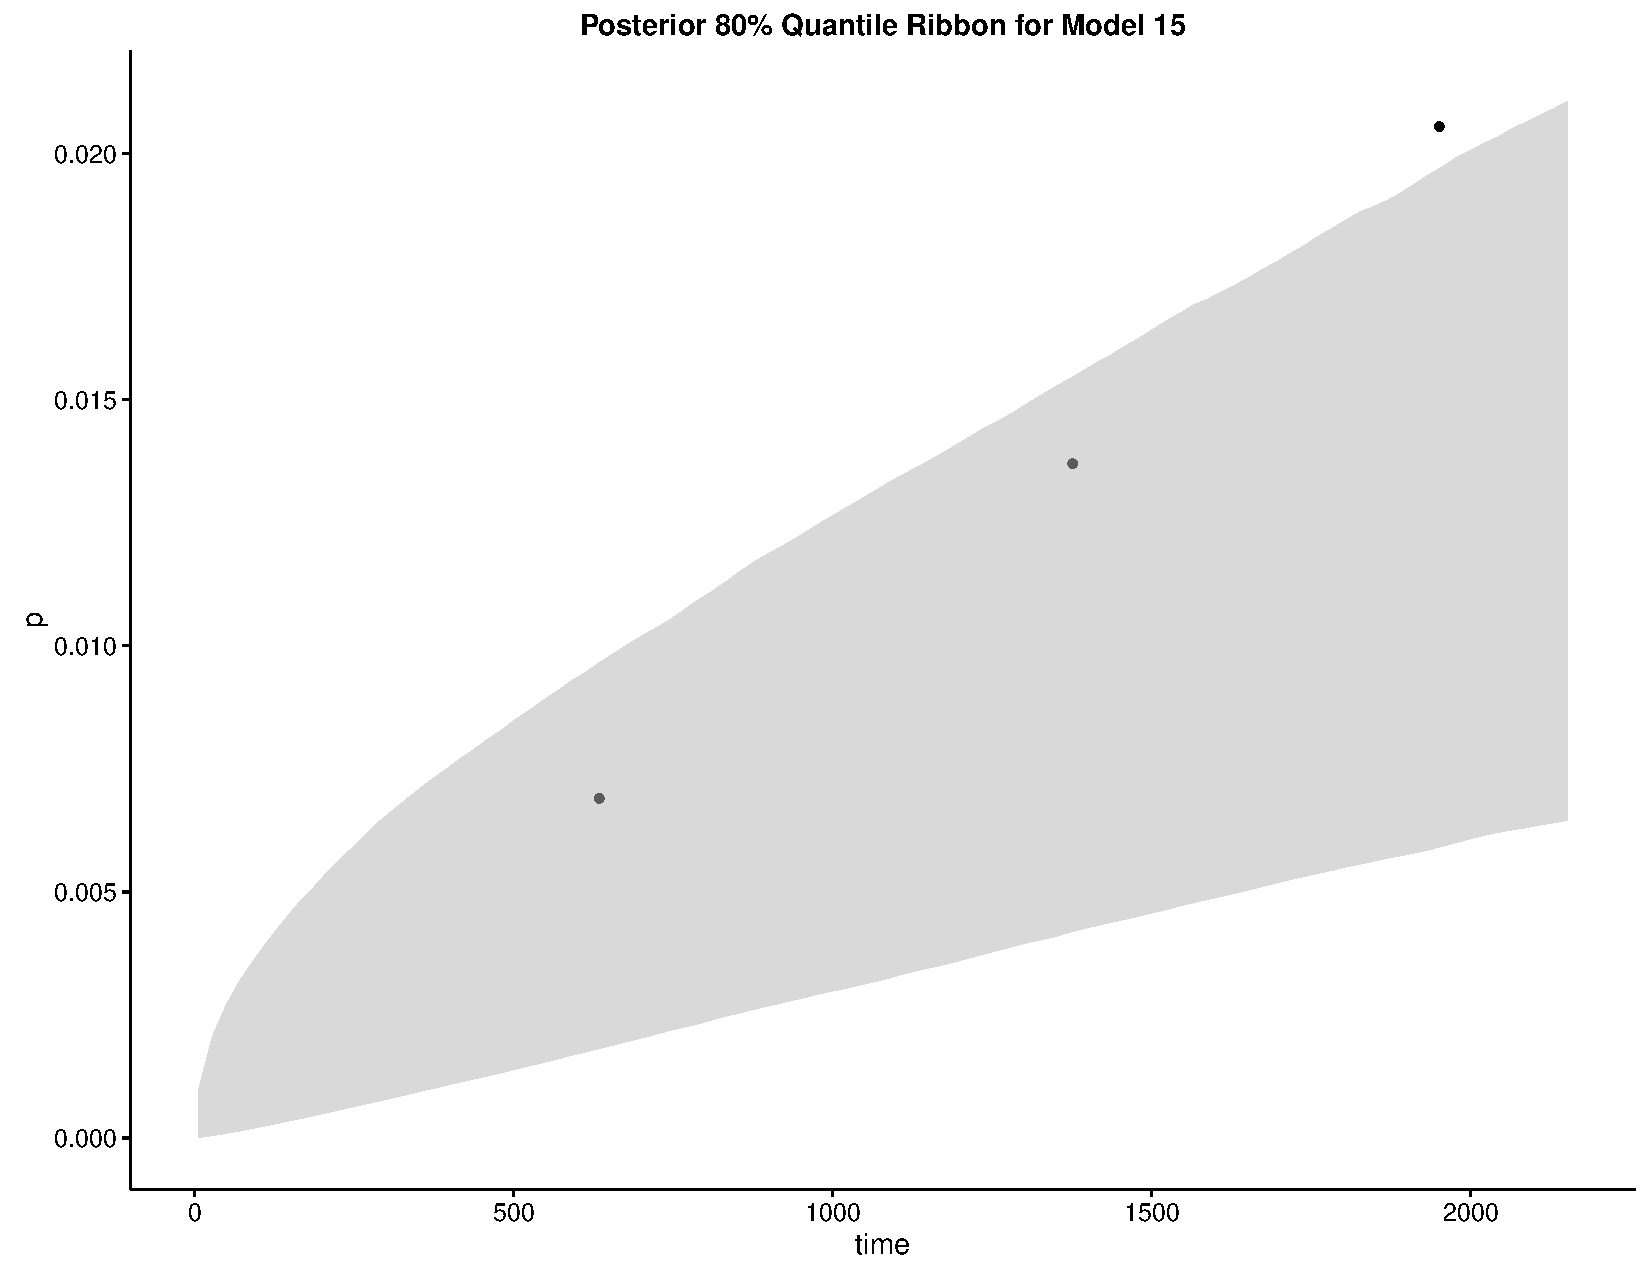
\includegraphics[width=\textwidth]{plot3.pdf}
  \end{minipage}
  \hfill
  \begin{minipage}[b]{0.4\textwidth}
    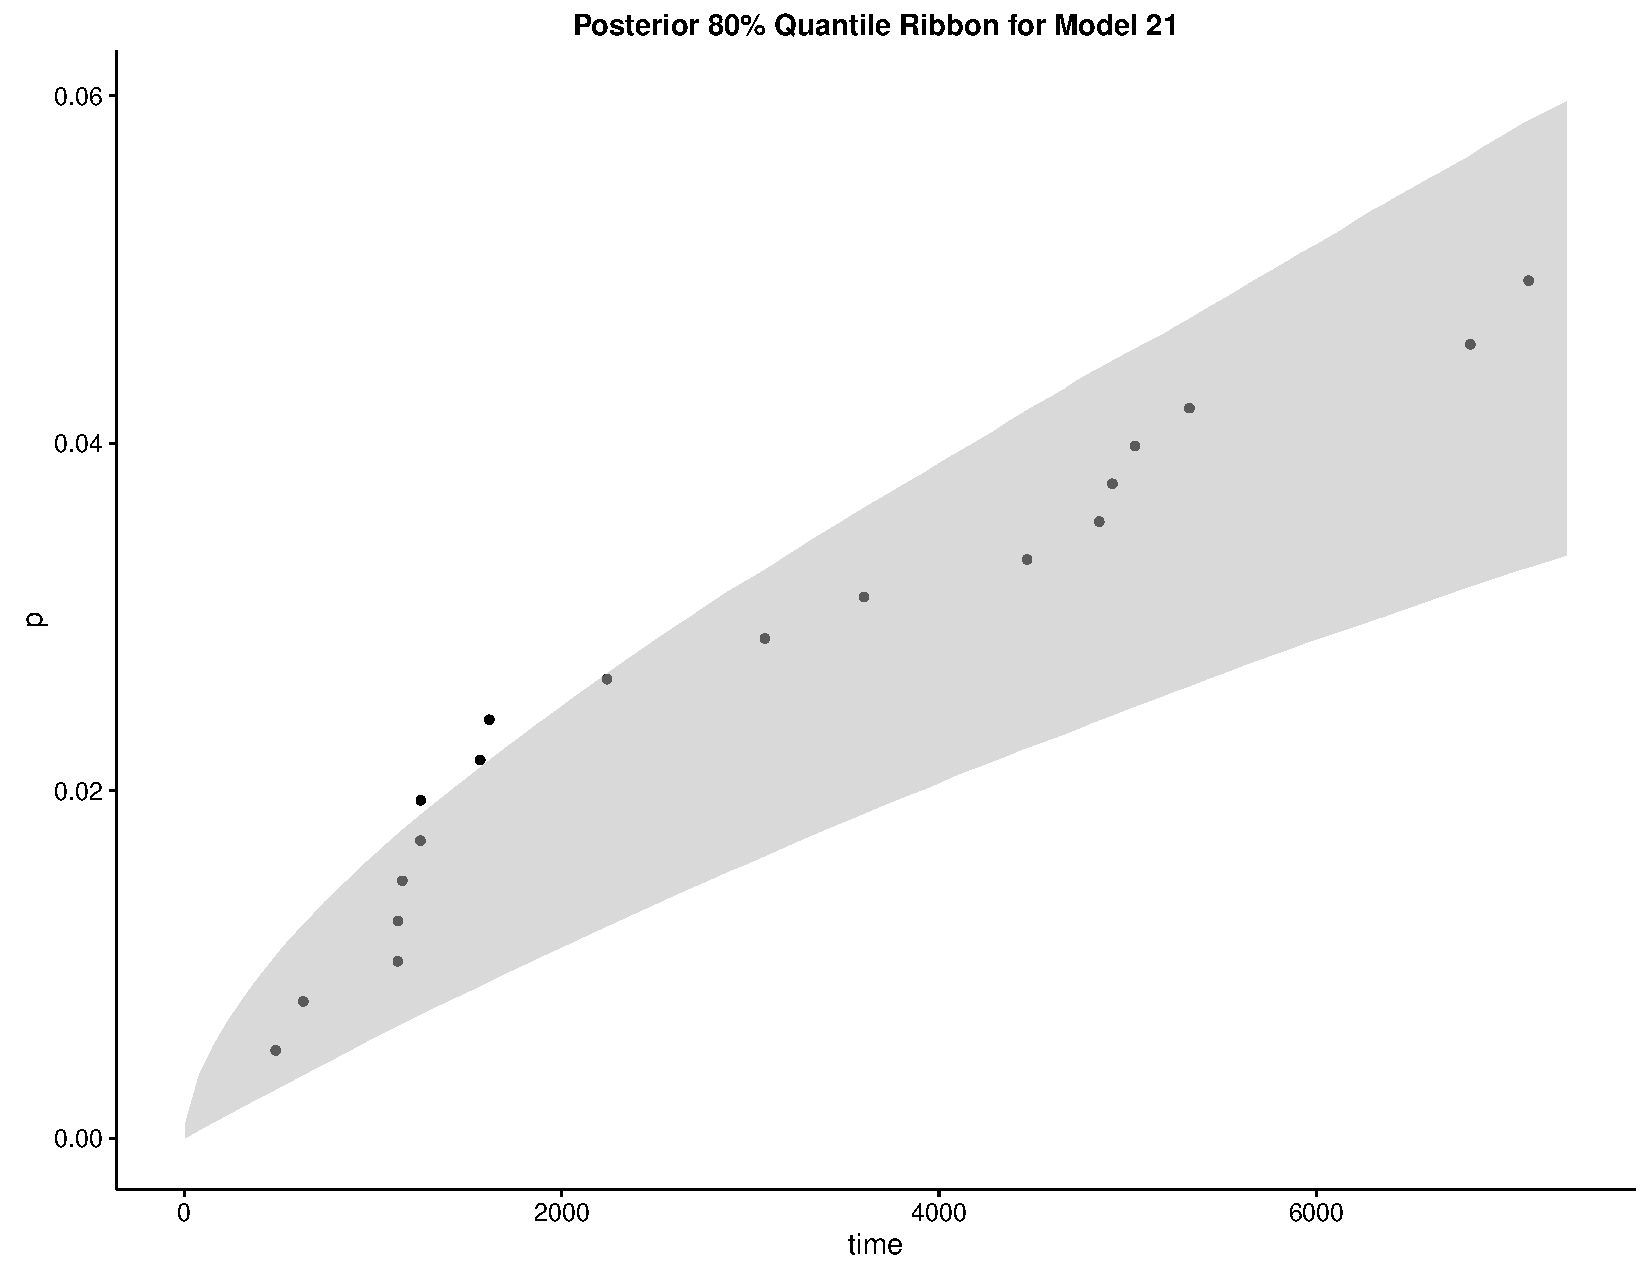
\includegraphics[width=\textwidth]{plot4.pdf}
  \end{minipage}
\end{figure}

When working with such a small number of failures, the Bayes hierarchical framework is advantageous as it pools information from across brands to get more precise estimates of the individual model parameters.  Unfortunately, even when pooling information, with relatively few failures it is still difficult to statistically differentiate the reliability between most hard drive brands. It is encouraging, though, that the Weibull model does seem to fit the data quite well: especially for Model 11, which has the most observed failures.  As additional information is collected, it should become easier to differentiate across brands as the uncertainty around the model parameters will decrease.\\ 

Going forward it would be smart for Backblaze to incorporate accelerated testing (perhaps via elevated temperatures) to increase the number of failures from their tests.  And for us statisticians, it would be interesting to compare the Bayes results to estimates obtained from a standard frequentist approach where Weibull models are fit to each brand using maximum likelihood estimation.


\bibliographystyle{plain}
\bibliography{bibliography} 
\clearpage
\begin{appendices}
\section*{Stan model}
{\scriptsize
\begin{verbatim}
data {
  int<lower=0> N_obs;
  int<lower=0> N_cens;
  int<lower=0> N_tr_obs;
  int<lower=0> N_tr_cens;
  int<lower=0> M;

  // right endpoints
  real<lower=0> y_obs[N_obs];
  real<lower=0> y_cens[N_cens];
  real<lower=0> y_tr_obs[N_tr_obs];
  real<lower=0> y_tr_cens[N_tr_cens];

  // truncation points
  real<lower=0> t_obs[N_tr_obs];
  real<lower=0> t_cens[N_tr_cens];

  // explanatory variable
  int<lower=1, upper=M> x_obs[N_obs];
  int<lower=1, upper=M> x_cens[N_cens];
  int<lower=1, upper=M> x_tr_obs[N_tr_obs];
  int<lower=1, upper=M> x_tr_cens[N_tr_cens];

  // quantile to set prior on
  real<lower=0, upper=1> p;
}
transformed data{
  real<lower=0> Q;
  Q <- -1.0 * log(1-p);
}
parameters {
  vector[M] log_tp;
  vector[M] log_sigma;
  real m1;
  real<lower=0> C1;
  real m2;
  real<lower=0> C2;
}
transformed parameters {
  vector<lower=0>[M] eta;
  vector<lower=0>[M] beta;
  beta <- exp(-1.0 * log_sigma);
  for(i in 1:M){
    eta[i] <- exp(log_tp[i])/(Q^(1/beta[i]));
  }
}
model {
  for(i in 1:N_obs){
    y_obs[i] ~ weibull(beta[x_obs[i]], eta[x_obs[i]]);
  }

  for(i in 1:N_cens){
    increment_log_prob(weibull_ccdf_log(y_cens[i], beta[x_cens[i]], eta[x_cens[i]]));
  }

  for(i in 1:N_tr_obs){
    increment_log_prob(        weibull_log(y_tr_obs[i], beta[x_tr_obs[i]], eta[x_tr_obs[i]]));
    increment_log_prob(-1.0 * weibull_ccdf_log(t_obs[i], beta[x_tr_obs[i]], eta[x_tr_obs[i]]));
  }

  for(i in 1:N_tr_cens){
    increment_log_prob(       weibull_ccdf_log(y_tr_cens[i], beta[x_tr_cens[i]], eta[x_tr_cens[i]]));
    increment_log_prob(-1.0 * weibull_ccdf_log(    t_cens[i], beta[x_tr_cens[i]], eta[x_tr_cens[i]]));
  }

  log_tp ~ student_t(5, m1, C1);
  log_sigma ~ normal(m2, C2);

  //priors (improper prior on m1 and m2)
  C1 ~ cauchy(0, 10);
  C2 ~ cauchy(0,10);}
  }
  \end{verbatim}
  }
\end{appendices}
\end{document}

